%%% Thesis Introduction --------------------------------------------------
\chapter{Introduction}
\ifpdf
    \graphicspath{{Introduction/IntroductionFigs/PNG/}{Introduction/IntroductionFigs/PDF/}{Introduction/IntroductionFigs/}}
\else
    \graphicspath{{Introduction/IntroductionFigs/EPS/}{Introduction/IntroductionFigs/}}
\fi

In 1965 Gordon E. Moore predicted that the power of computing hardware will double every two years \citep{Moore:1965uj}. This exponential growth of digital technology, widely known as Moore's law still holds true even today \citep{Robison:2012ij}.  The biennial doubling of computational power allowed for cheap, powerful digital devices and had an immense impact on all aspects of human life. Although remarkable in itself, this growth has recently been surpassed by the pace of DNA\nomenclature{DNA}{deoxyribonucleic acid} sequencing technology \citep{Dewitt:2012dq}. 

The amount of nucleotide sequence information we now have on genomes of living organisms exceeds current storage and retrieval capacities \citep{HsiYangFritz:2011iy}. However, to quote John Naisbit, an author in future studies, ``we are drowning in information, but starved for knowledge". The human genome project revealed that less than 5\% of genomic sequence codes for proteins,  a large proportion being unannotated and commonly referred to as ``junk'' DNA \citep{lander:2001hk}.  From an evolutionary perspective this lack of apparent function makes little sense, since it is too costly to maintain and duplicate nonfunctional parts of DNA with no benefits for survival.  In addition, recent sequencing projects revealed that about 80\% of the human genome produces RNA transcripts that never code for functional proteins \citep{Consortium:2012db}. 

\begin{landscape}
\begin{figure}[hbtp!]
\begin{center}
\includegraphics[width=22cm]{timeline}
\caption[History of genomics and non-coding RNAs]{Major discoveries in the history of genomics and non-coding RNAs.}
 \label{fig:timeline}
\end{center}
\end{figure}
\end{landscape}

It is now clear that these non-coding RNAs are implicated in a vast range of biological processes, from transcriptional regulation, chromatin maintenance to development and disease \citep{Amaral:2008cb}. However, the importance of this diverse set of molecules is only recently being appreciated. In the next chapter I will discuss multiple advances in genome biology and sequencing technology that have been necessary to fully ascertain their role (Figure \ref{fig:timeline}).

\section{RNA world: ancient past or hidden present}

Nucleic acids were discovered in 1869 by a German physician Friedrich Miescher \citep{Miescher:1869tn}. After about 70 years and multiple advances in organic chemistry and biochemistry it was generally accepted that RNA is not merely ``yeast nucleic acid'', a DNA version specific to certain species or just to cytoplasm \citep{Allen:1941ib}. Proteins were considered the main molecules of heredity at the time, due to the greater complexity of amino-acid versus nucleotide content  \citep{Darnell:2011wt}. Surprisingly, RNAs\nomenclature{RNA}{ribonucleic acid} had been identified as the sole nucleic acid of certain viruses as early as 1937 \citep{Bawden:1937ua}, before the confirmation of DNA acting as the carrier of information across bacterial strains \citep{McCarty:1946ul}. 

Further advances in crystallography and biochemistry brought the discovery of DNA structure in 1953 \citep{Watson:1953vf} and the central dogma of molecular biology in 1958: transfer of biological information occurs from DNA via RNA to protein \citep{CRICK:1958ws}. Several coding and non-coding RNAs were identified to play an essential role in the process. The coding messenger RNAs (mRNAs) were shown to give instructions for protein synthesis \citep{BRENNER:1961ve}, with the non-coding transfer RNAs (tRNAs)\nomenclature{tRNA}{transfer RNA} \citep{CANELLAKIS:1957ts} translating mRNA code into amino-acids with the help of ribosomes and ribosomal RNAs (rRNAs)\nomenclature{rRNA}{ribosomal RNA} \citep{SCHERRER:1963uj}. Later, other non-coding RNAs were also implicated in protein synthesis. Small nuclear RNAs (snRNAs)\nomenclature{snRNA}{small nuclear RNA} \citep{Lerner:1979ur} were found to be involved in protein production by removing introns, the non-coding parts of mature mRNA precursors. Furthermore, small nucleolar RNAs (snoRNAs)\nomenclature{snoRNA}{small nucleolar RNA} chemically modify rRNAs and tRNAs during their maturation \citep{Weinberg:1968uk,Hughes:1991tc}. Irrespectively of these major advances in RNA biology, the primary function assigned to RNAs was to be the crucial carrier of information from DNA to protein. It took another two decades before the regulatory non-coding functions of RNA were discovered.

The perception of RNA changed in the early 1980s with the rise of molecular biology techniques and the discovery of ribozymes --- the RNA molecules that perform enzymatic function. The first ribozymes were observed in the laboratories of Altman and Cech, who received a Nobel prize in 1989 for ``Discovery of catalytic properties of RNA'' \citep{Altman:2000bx}. Altman studied the nucleoprotein RNAse P, a tRNA processing enzyme, and realised that the active component is not protein but RNA \citep{GuerrierTakada:1983vi}. At the same time Cech was working on rRNA specific ``intervening sequences'' that excised themselves out of the long primary transcript in a protein free system \citep{Kruger:1982wk}. 

Based on the enzymatic properties of RNA, the ``RNA world'' hypothesis was suggested \citep{Gilbert:1986cq}. This hypothesis presumed that in the history of life on earth RNA molecules were likely the first biological entities. It is not known how the first molecules of RNA were formed, especially since they are prone to hydrolysis and need catalysis to form stable polymers \citep{Lindahl:1967wc}. However, recapitulations of prebiotic biochemistry resulted in formation of stretches of RNA by catalysis with inorganic materials such as lead (Pb\textsuperscript{2+}) metal ions \citep{Sleeper:1979un} or molecules of clay \citep{Ertem:2000gl}. In fact, the latter study managed to produce oligonucleotides of up to length 50 in a matter of days. Though this may seem short, it was shown that 165 nt long RNAs can already perform complex template based RNA polymerisations \citep{Johnston:2001tl}. Details of the initial RNA formation may remain unknown, but the RNAs of today are still capable of  storing the information, as well as performing enzymatic functions or making helper molecules \citep{Maxam:1977vy}. The last affirmation of the importance of RNA in the DNA-RNA-protein paradigm came from the ribosome crystal structure, which presented evidence that the catalytic engine of the protein synthesis machinery is RNA. Interestingly, proteins were found to provide just a scaffold for the function of rRNAs \citep{Nissen:2000wo}. 

These discoveries separated RNA molecules from the simple protein making intermediaries, though the full repertoire of functions that the non-coding RNAs perform was yet to be discovered. Since the late 1980s and the technological advances of recombinant DNA, DNA sequencing and sequence amplification, a number of diverse RNA molecules has been identified with their own unique biological functions. The first large family of the non-coding RNAs was microRNAs (miRNAs) \citep{Lee:1993ev}. These 18-23 nucleotide (nt)\nomenclature{nt}{nucleotide} non-coding RNAs regulate the expression of multiple mRNAs by diminishing the rate of translation \citep{Lee:1993ev, Saxena:2003tk} as well as reduce the stability of transcripts \citep{Orban:2005kj}. Investigation of miRNA\nomenclature{miRNA}{microRNA} function on global RNA expression was supported by the establishment of high throughput transcriptomic platforms such as DNA microarrays, accompanied by the advances in computational biology \citep{Lim:2005cd}. MicroRNAs partly share the same function and biogenesis as other RNAs that regulate expression. One example are the small interfering RNAs (siRNA)\nomenclature{siRNA}{short interfering RNA} \citep{Hamilton:1999dy} that are a major part of the RNA interference response (RNAi)\nomenclature{RNAi}{RNA interference resonse}  with a further function in the regulation of viruses as well as transposable elements \citep{Tuschl:1999wa}. The rise of high throughput sequencing technologies allowed for the discovery of PIWI protein interacting RNAs (piRNAs)\nomenclature{piRNA}{PIWI protein interacting RNAs}. These 24-32 nt small non-coding RNAs regulate transposable elements and maintain genome stability in the germ line throughout the animal kingdom \citep{Vagin:2006cs, Grivna:2006p676, Aravin:2006p384}. Finally, a set of long non-coding RNAs (lncRNA)\nomenclature{lncRNA}{long non-coding RNA} were identified as a class in 2002 \citep{Okazaki:2002wv} even though some lncRNA such as H19 and Xist were known since early 1990s \citep{Brannan:1990vk, Brockdorff:1992tu}. These RNAs are characterised by their length and low coding potential and they assume a broad range of functions in transcriptional regulation and chromatin modification \citep[review in][]{Rinn:2012fh}. In addition to the previously mentioned large non-coding RNA (ncRNA)\nomenclature{ncRNA}{non-coding RNA} categories, multiple other types were discovered: vault RNAs \citep{Kedersha:1986vi, Gopinath:2010fa} that are probably involved in resistance to foreign small molecules, or more recent transcription initiation RNAs (tiRNA)\nomenclature{tiRNA}{transcription initiation RNA} \citep{Taft:2009jp} and enhancer associated RNAs (eRNA)\nomenclature{eRNA}{enhancer RNA} \citep{Kim:2010bl}, involved in transcription regulation.
 
This work will focus on computational approaches in studies of biogenesis and function of non-coding RNA molecules. More specifically, these results cover biogenesis of embryonic and adult piRNAs in mammals, as well as the detection of miRNAs in genome-wide expression datasets. To this end, two classes of non-coding RNAs, miRNAs and piRNAs will be discussed in greater detail, as well as the high throughput technologies required for their assessment.

	\section{MicroRNAs}

MicroRNAs are a class of small non-coding RNAs \citep{LagosQuintana:2001ir, Lee:2001un} involved in a wide range of processes from development  to cancerogenesis  \citep[reviewes in ][]{Kosik:2009fy, Zimmerman:2011kc}. The first miRNA (lin-4) was discovered in \textit{Caenorhabditis elegans}, where it was regulating the lin-14 protein by binding to its transcript in an antisense manner \citep{Lee:1993ev}. The miRNA field started only a few years later, with the discovery of \mbox{let-7} from \textit{C. elegans} that was conserved in all animals \citep{Ruvkun:2000dh} and c.22~nt RNA in plants \citep{Ruvkun:2000dh, Hamilton:1999dy}. Since then, a number of studies have identified details of the biogenesis and function of miRNAs in various biological processes.

	\subsection{Biogenesis of miRNAs}

The processing of mature miRNAs from their primary transcripts as well as the required protein machinery are similar for all animals. In the first step, RNA polymerase II (RNAP II) \citep{Lee:2004ia} produces a long genomic RNA precursor, called pri-miRNA containing a hairpin loop \citep{Hutvagner:2001fd}. Afterwards, nuclear proteins cut the pri-miRNA at the base of the hairpin into a 70 nt long pre-miRNA \citep{Lee:2002ei}. This is performed by Drosha, an RNAase III family protein that is accompanied by DGCR8 (vertebrates) or Pasha (invertebrates) \citep{Denli:2004do} and releases the hairpin structure with a typical $5\textprime$ phosphate and $3\textprime$ overhang of two nucleotides \citep{Lee:2002ei}. The final step to produce the mature miRNA involves the export from the nucleus by Exportin V \citep{Yi:2003gz} and processing of pre-miRNAs by an endonuclease called Dicer \citep{Hutvagner:2001fd}. The mature miRNA is then incorporated into the RNA induced silencing complex (RISC)\nomenclature{RISC}{RNA induced silencing complex}. This complex contains a set of proteins that help miRNAs to attenuate protein synthesis and mRNA expression \citep{Hammond:2000kr}. 


\begin{figure}[hbtp!]
\begin{center}
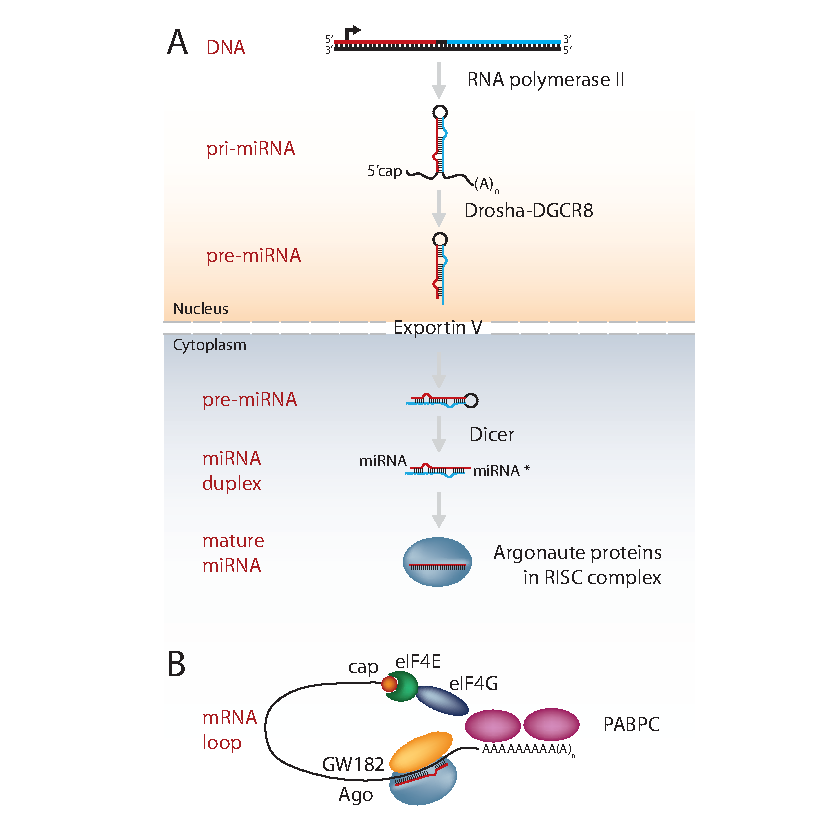
\includegraphics[width=14cm]{miRNAs}
\caption[Biogenesis of miRNAs]{Biogenesis of miRNAs and influence on translation and transcript stability. A. MicroRNA primary transcripts are transcribed by RNAP II into pri-miRNAs with a hairpin loop. After the hairpin has been processed by the Drosha and DGCR8 proteins (Pasha in invertebrates) into pre-miRNAs, it is exported from nucleus by Exportin V. Afterwards, the loop is processed by Dicer, followed by the separation of the mature and the passenger (star) strand. The mature miRNA then binds to the AGO proteins in the RISC complex. B. MicroRNAs control translation and transcript stability by influencing the mRNA loop formation. MicroRNAs lead the RISC complex with GW178 to the transcript. GW178 interferes with the interaction of PABPC with eIF4G which slows down translation. This interference also decreases the number of transcript bound PABPC proteins that protect the polyadenylated tail from exonucleases is decreased, decreasing the transcript stability. \citep{Huntzinger:2011ik}.}
\label{fig:miRNAs}
\end{center}
\end{figure}

The RISC complex contains various Argonoute (AGO)\nomenclature{AGO}{Argonaute} proteins that are guided by small RNAs such as siRNAs and miRNAs to decrease expression of multiple mRNA targets \citep{Meister:2004ha}. The targeting is performed through base pairing between the guide molecule and its target, mainly through a small number of miRNA nucleotides at their $5\textprime$ end termed the ``seed region'' \citep{Lewis:2003ig}. The mature miRNA guides the primed RISC complex to the complementary mRNA loci termed ``target sites'' or miRNA recognition elements (MREs)\nomenclature{MRE}{miRNA recognition elements} \citep{Hutvagner:2001fd}. Target sites are mainly located in the $3\textprime$ untranslated regions (UTRs)\nomenclature{UTR}{untranslated region}, though other parts seem to have importance as well \citep{Bartel:2009fh, InhanLee:2009em}. Depending on the extent of miRNA binding to the target sites, the influence over expression can be quite different. Perfect complementarity leads to direct target cleavage \citep{Yekta:2004ip} and is commonly referred to as RNA interference (RNAi). This is characteristic for siRNAs and is also the main mechanism of miRNAs in plants \citep{Llave:2002uv}. Otherwise, the imperfect miRNA-mRNA binding can influence a large number of targets by both inhibition of mRNA translation \citep{Lee:1993ev, Saxena:2003tk} and decrease of mRNA stability \citep{Orban:2005kj}. Research is still performed to establish the extent and temporal dynamics of each of the previous two processes.
    	
\nomenclature{A, T, G, C, U}{Adenine, Thymine, Guanine, Cytosine, Uracil} 
	
	
	\subsection{MicroRNA mode of action}
	\label{sec:mirna_effects}
	
The main players and processes in the inhibition of mRNA translation by miRNAs have been well described. The miRNAs act on mRNA loop formation (Figure \ref{fig:miRNAs}), whereby $5\textprime$ and $3\textprime$ ends of mRNAs come into proximity, promoting interactions of the $5\textprime$-cap- and the poly(A)-binding proteins and a more efficient translation \citep{Wells:1998jo}. Although miRNAs could act on several stages of translation: initiation \citep{Pillai:2005fx}, elongation \citep{Lee:1993ev, Petersen:2006eb} and protein degradation \citep{Nottrott:2006ju}, not all observations can be fit into a same model. The predominant view is that during the initiation phase proteins from the RISC complex act as $5\textprime$ mRNA cap binding proteins and compete with translation initiation factors \citep{Pillai:2005fx, Kiriakidou:2007il}. This observation has been further confirmed by the lack of miRNA translation silencing upon modification of $5\textprime$ mRNA cap \citep{MotoakiWakiyama:2007fw}, as well as by increased concentration of $5\textprime$ cap binding proteins \citep{Mathonnet:2007ev}. The GW182 protein seems to play a crucial role in this process \citep{Zekri:2009dl}. This RISC complex protein is required for miRNA-mediated gene silencing by competing with the initiation factor eIF4G for binding to the poly(A)-binding protein PABPC.

Besides influencing the translation process, miRNA also decrease the stability of transcripts. The first evidence came from transfection of two miRNAs, miR-1 and miR-124, into cells within which they are normally not expressed \citep{Lim:2005cd}. This  resulted in down-regulation of transcripts containing complementary binding sites. Similarly, levels of miR-430 targets increased in cells in which this miRNA is inhibited \citep{Giraldez:2006gr}. On the mechanistic level, miRNAs seem to promote deadenylation of the mRNA targets, stimulating faster degradation \citep{Giraldez:2006gr, AnaEulalio:2009eh}. This occurs through the previously mentioned GW182 protein that binds miRNAs in the RISC complex and recruits deadenylase complexes to $3\textprime$UTRs of miRNA targets \citep{Braun:2011bo}. Afterwards, the mRNA target is degraded by the enzymes involved in the cellular $5\textprime$-to-$3\textprime$ mRNA decay pathway \citep{BEHMANSMANT:2006fi}. In this pathway, deadenylated \mbox{mRNAs} are decapped by the enzyme DCP2, and ultimately degraded by the major cytoplasmic $5\textprime$-to-$3\textprime$ exonuclease XRN1 \citep{REHWINKEL:2005hp}.

Despite the growing knowledge in the field of miRNA effector functions, it is still unresolved whether miRNA act through translation inhibition or decrease of mRNA stability. In a recent study it was stated that 84\% of changes in protein amount are explicable by the miRNA induced mRNA decay \citep{Guo:2010kh}. On the other hand, translation inhibition can sometimes occur without an influence on expression or even before it \citep{Bazzini:2012jka}. Therefore, it is hypothesised that the same miRNA primed mechanism probably influences independently both mRNA levels and translation \citep{Boland:2011ik}. The function of the intermediary is probably held by GW182 and its two protein binding domains \citep{Fukaya:2011fm} that can influence both expression through PAPBC  \citep{Zekri:2009dl} and translation through the CCR4-NOT proteins \citep{Chekulaeva:2011et} at the same time. 
   
   
 	\subsection{Identification of miRNA targets}
	\label{ref:miRNA_targets}

The mode of action of miRNAs is still disputed, but it is clear that miRNAs influence hundreds of genes at the mRNA and protein levels \citep{Lim:2005cd, Baek:2008ir}. Therefore, identification of individual miRNA targets is performed by an initial identification of potential miRNA-mRNA candidates by genetic, biochemical or computational methods \citep[review in][]{Thomson:2011hc}, which is followed by validation of the predicted interactions \citep[review in][]{Vasudevan:2012cw}. 
	
	Genetic methods for the identification of miRNA-mRNA pairs involve either the mRNA or protein measurements after a perturbation of miRNA level such as over-expression or inhibition Over-expression of miRNAs can be achieved by introducing miRNA hairpin precursors in vectors that produce stable amounts of miRNA \citep{Brummelkamp:2002vx}. However, this approach is problematic since it increases the miRNA amount to artificially high levels that can oversaturate Exportin V or RISC complex proteins and outcompete other miRNAs \citep{Grimm:2006jz}. A further improvement of the system was achieved with lentiviral vectors with pre-miRNAs, the levels of which are more readily controlled \citep{Stegmeier:2005kf}. On the other hand, inhibition of miRNAs is a more controlled way of perturbing miRNAs and can be performed with various silencing approaches. The cells can be transfected with either synthetic miRNA-antisense oligonucleotides like antagomirs \citep{Krutzfeldt:2005ch} and anti-miRs \citep{Elmen:2008iz}, or with vectors expressing antisense miRNA \citep{Ebert:2007ch}.  Both over-expression and inhibition approaches are followed by observations of genome-scale changes either at the expression level through microarrays \citep{Lim:2005cd} and RNAseq \citep{Deng:2011fu}, or at the protein level through stable isotope labelling by amino acids in cell culture (SILAC) \citep{Vinther:2006dk, Selbach:2008hx}. The major drawback of all these methods is that the number of identified mRNA or proteins is quite large and secondary effects of the observed changes cannot be excluded. For that purpose, more specific biochemical approaches have been developed.
	
	The biochemical methods attempt to capture only the primary miRNA targets by immunoprecipitation of RISC proteins and the attached RNAs. Early attempts were directed at the capture of the RISC components \citep{Easow:2007co,Karginov:2007ki} followed by microarray identification of bound RNAs. Though these methods capture RISC-bound RNAs, they are not necessarily native, since these approaches involve a cell lysis step before the RNA assessment. This has been circumvented by exploiting the property of proteins to crosslink bound RNA when submitted to UV in vivo. The crosslinking can be followed by immunoprecipitation (CLIP) to isolate the protein of interest \citep{Ule:2003ja}. The first CLIP method on Ago immunoprecipitates aimed at identifying at the same time both the miRNA and its mRNA target through high throughput sequencing (HITS-CLIP) \citep{Chi:2009ht}. Follow-up methods were developed that surpassed the limits of CLIP such as low efficiency of crosslinking and the lack of the crosslink site information. PAR-CLIP  \citep{Hafner:2010kr} uses photoactivatable ribonucleosides that facilitate cross linking and allows for identification of the cross linking sites through a T to C conversion that occurrs at these loci. On the other hand, iCLIP \citep{Konig:2010ca} identifies the cross link site and reduces the impact of reduced library complexity that occurs through PCR amplification in the usual CLIP procedures. The first step of iCLIP involves a circularisation of all the cross linked reads and is followed by reverse transcription that stops at the cross linking sites where amino acids are attached to RNAs. The sequences therefore start with the cross linking site, and by using barcodes in the sequencing adapters it is also easier to discern the amplification products from the unique sequences. The optimisation of the previously mentioned CLIP methods is still ongoing, but the technology allows for an experimental approach in miRNA target identification that is currently largely independent of computational predictions. 

\begin{figure}[hbtp!]
\begin{center}
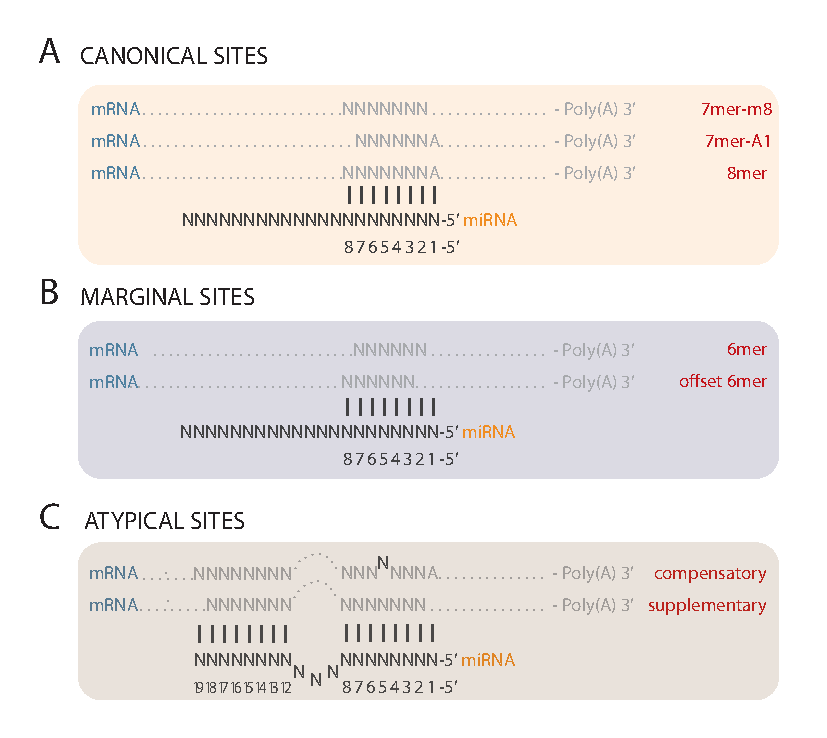
\includegraphics[width=14cm]{seeds}
\caption[Classification of the miRNA-mRNA binding sites]{Classification of the miRNA-mRNA binding sites. The order from top to bottom of the canonical, marginal and atypical categories reflects the decreasing silencing efficiency \citep{Bartel:2009fh}. A. The canonical sites have the strictest binding between the miRNA and mRNA at the seed region (nucleotides 2-8 from $5\textprime$ miRNA end), and can be either 7 or 8 nt long. The most efficient silencers are 8mers, followed by 7mer-m8 and 7mer-A1. B. Marginal sites are 6 nt long and less efficient in silencing, though they are equally abundant. C. The atypical sites rely on binding between miRNA and mRNA outside of the seed region, for more than four (compensatory) or more than three base pairs (supplementary).}
 \label{fig:seeds}
\end{center}
\end{figure}

Computational methods for miRNA target prediction use a combination of sequence, thermodynamic features and conservation of miRNAs and mRNAs to go beyond the limits of experimental procedures. For a computational analysis the sequence of miRNA-mRNA interfaces seems the easiest property to exploit. However, in mammals the position and the extent of binding can vary \citep{Bartel:2009fh}. The majority of pairing between a miRNA and its target is achieved through complementarity with the miRNA $5\textprime$ seed region of nucleotides 2-8 \citep{Lewis:2003ig}. Beside this canonical 7mer pairing, others have been observed (Figure \ref{fig:seeds}) and involve different position and length at the $5\textprime$ end of miRNA, as well as involving other miRNA parts with various degrees of matches and mismatches \citep{MWitkos:2011gj}. Sequence information can also be employed to predict thermodynamic energy of a miRNA-mRNA duplex, or estimate the importance of sequence elements by their conservation in evolution \citep{Enright:2003fj}. 

Multiple algorithms have been developed that use the previously mentioned properties to varying degrees. The first computational target prediction used validated miRNA targets in Droposhila \citep{Stark:2003jb} and was followed by miRanda \citep{John:2004ke}. miRanda used the Smith-Waterman approach \citep{Smith:1981up} to align whole miRNA region with the potential target sites, but weighting results more strongly for matches within the seed region and allowing for mismatches. High-scoring targets were then filtered on the free energy of miRNA-mRNA duplex and conservation predictions. Other methods emphasise different miRNA properties, such as conservation in PicTar \citep{Krek:2005er}, or train their datasets on validated targets as in microT \citep{Kiriakidou:2004kc}. Currently the most popular algorithm is TargetScanS. It requires perfect binding matches within the seed region, in the so called ``canonical sites'' and ``marginal sites'' (Figure \ref{fig:seeds}) \citep{RobinCFriedman:2009km}. It also uses thermodynamics based modelling and performs conservation analysis on human, mouse, rat, dog and chicken \citep{RobinCFriedman:2009km}. However, this algorithm still predicts only 49\% of targets validated from proteomic studies \citep{MWitkos:2011gj}, pointing to the limits of computational miRNA target predictions. On the other hand, methods have been devised that assess enrichment of miRNA targets in the genes lists acquired from the experimental data such as GeneSet2miRNA \citep{Antonov:2009gx},  DIANA-mirExTra \citep{Alexiou:2010bt} and Sylamer \citep{vanDongen:2008cb}. An application of the Sylamer algorithm in detection of miRNA influence on expression datasets will be discussed in Chapter \ref{sec:Chapter4}.
	
After the initial miRNA-mRNA candidates have been established, they have to be validated by one of the following three approaches. In the first one, a cell line is transfected with the bioluminescent protein luciferase, containing the target site for a miRNA of interest in the $3\textprime$ UTR \citep{Zeng:2003ka, Vasudevan:2007by}. The miRNA precursors are then depleted with short interfering RNAs and the target site is confirmed if the luciferase signal was attenuated and if the luciferase with mutated target sites in the $3\textprime$ UTRs is unaffected. After the miRNA levels have been restored by addition of synthetic mature microRNA, the target expression levels are measured to confirm miRNA repression \citep{Vasudevan:2007by}. Similarly, interaction of miRNA with mRNA can be blocked by the previously mentioned antagomirs \citep{Krutzfeldt:2005ch} and anti-miRs \citep{Elmen:2008iz} that can be specifically designed to block only certain mRNAs from miRNA influence. Finally, both the target sites on mRNA can be mutated, followed by a treatment by complementarily mutated miRNAs to rescue the expression levels. 
	
	 	\subsection{The impact of miRNAs}
		\label{sec:miRNA_impact}

Although the first miRNAs have been discovered 20 years ago, it was only in the last 10 years that a vast number of crucial discoveries have been reported \citep{Bartel:2009fh,Vergoulis:2012dk}. This explosion of miRNA related research is largely a consequence of the combination of the rise of new technologies (see Chapter \ref{sequencing}) that gave us sequence information of genomes, high throughput assessment of miRNAs and their targets, as well as computational biology methods  \citep{Lu:2005fx, Ruby:2006bc}. The current release of miRBase (v. 19) \citep{Kozomara:2011es} contains information on more than 25.000 mature miRNAs in 193 species, while over 65.000 entries can be found in Tarbase, the database of validated miRNA-mRNA interactions \citep{Vergoulis:2012dk}. 

MicroRNAs are involved in a multitude of biological process based on their capability to attenuate expression of hundreds of genes at a time \citep{Lim:2005cd, Baek:2008ir}. The effects of miRNAs on individual genes are usually on a small scale \citep{Bartel:2009fh}, but a cumulative effect of such small modifications can result in a change of a developmental plan. For example, introduction of miR-124 to fibroblasts managed to convert them to active neurons \citep{Yoo:2011gt}. This miRNA mode of action can be observed in development \citep[review in][]{Kosik:2009fy}) as well as in other processes such as immune response \citep{Vigorito:2007hk} and cancerogenesis \citep[review in ][]{Zimmerman:2011kc}. Recently, other unexpected miRNA functions have been observed: from exchange of information between cells  \citep{Zhang:2010hd} to receptor-binding in immune response \citep{Lehmann:2012fe}. Such diverse repertoire of functions allows miRNAs to act as both markers of disease \citep[review in][]{Teplyuk:2012dq} and therapeutics \citep{Czech:2011it}. 

Similar to miRNAs, piRNAs were not detected for a long time despite being crucial in silencing of another ubiquitous source of transcripts --- transposable elements. These small non-coding RNAs will be discussed in the next section. 

\section{PIWI-protein interacting RNAs}	
\label{piRNAs}
Transposable elements (TEs) or transposons \citep{McClintock:1950wz} are genomic parasites (``selfish genes'' that are characteristic for all domains of life \citep{Llorens:2007df}. They are characterised by their ability to create their copies elsewhere in the genome (``copy-paste''), or simply relocate their own sequence (``cut-paste''). Alhough it is presumed that some of them are beneficial for genome evolution \citep{Brandt:2005jl}, they induce genome instability by insertional mutations and by providing substrates for additional recombination events \citep{Deininger:2003wk}. Some prokaryotes have developed a defence against them through the CRISPR system (Clustered Regularly Interspaced Short Palindromic Repeats)  \citep{Jansen:2002ve, Mojica:2005hk}. This genetic defence mechanism allows bacteria to store information on viruses and mobile genetic elements it encountered and uses it to target their DNA in the future \citep{Bolotin:2005gj}. Other defence mechanism involve RNAi systems with AGO proteins  \citep{Song2:2004ge} that have also been implicated in the control of mobile genetic elements from prokaryotes, unicellular organisms to plants and animals  \citep{Makarova:2009kq, Djikeng:2001um, Hamilton:1999dy, Aravin:2003ht}. Some species of plants \citep{Mosher:2008ef} and animals \citep{Brandt:2005jl,Aravin:2008kz} employ DNA methylation to control transposons, since it can silence the expression of chromatin regions \citep{McGhee:1979tz}.

	Animals use small non-coding piRNAs and DNA methylation to target transposable elements, but their action is restricted to the germ-line cells. The germ-cell genomes need special protection since their information is directly transmitted to the offspring. Furthermore, in some species whole genomes undergo demethylation that derepresses silenced TEs \citep{Tada:1997kw,Mayer:2000dl}. In the following section general properties and biogenesis of piRNAs will be discussed in greater detail.
	
\subsection{Discovery of piRNAs}

PIWI-interacting RNAs were first described as ``repeat-associated small interfering RNAs'' (rasiRNAs) in 2001 based on their conserved function in control of retrotransposons in several species: \textit{Trypanosoma brucei} \citep{Djikeng:2001um}, \textit{Arabidopsis thaliana} \citep{Hamilton:1999dy} and \textit{Drosophila melanogaster} \citep{Aravin:2003ht}. The rasiRNAs are now considered just a subclass of the piRNAs specific for the regulation of transposable elements \citep{Brennecke:2007kfa}. After the definition of piRNAs as a novel class of non-coding RNAs in 2006 \citep{Vagin:2006cs, Aravin:2006p384, Watanabe:2006ij, Lau:2006ka, Girard:2006gu}, other characteristics have also been confirmed. 

First, their length was 24-31 nt, which made them separate from existing siRNAs and miRNAs that are often processed with Dicer proteins that are currently considered dispensable for piRNA production \citep{Vagin:2006cs}. Furthermore, piRNAs exhibit a strong propensity for a $5\textprime$-Uridine, characteristic of the \mbox{RNAse III} enzyme processing \citep{Aravin:2003ht}. Their $5\textprime$ end contains a monophosphate similar to other small non-coding RNAs. On the other hand, their $3\textprime$ end is specifically $2\textprime$-O-methylated, in contrast to animal miRNAs and siRNAs \citep{Kirino:2007iv}. Another property of piRNAs is that, when their sequence is aligned to the genome, they cluster to a set of genomic loci that can span up to few hundred kilobases \citep{Aravin:2007hw}. Finally, piRNAs are exclusively processed by the PIWI (P-element Induced Wimpy Testis) clade of the Argonaute protein family \citep{Aravin:2006p384}.

\subsection{Proteins involved in piRNA processing}
\label{sec:piwiprot}
PIWI (P-element induced wimpy testis)\nomenclature{PIWI}{P-element induced wimpy testis} proteins were first discovered in \textit{D. melanogaster} while examining germ-line stem cells through P-element mutagenesis \citep{Lin:1997un}. Mutations of these genes cause arrests in spermatogenesis and the consequential reduced size of gonads. Similar to other Argonaute proteins, PIWI homologues contain three domains,  PIWI, MID and PAZ (an abbreviation for Piwi/Argonaute/Zwille), essential for piRNA processing \citep{Cerutti:2000ut, Song:2004ge}. The PIWI domain contains the RNAase H fold that in some proteins performs endonucleolytic activity, also  termed ``slicing'' \citep{Song:2004ge, Parker:2005de, Gunawardane:2007ka}. Jointly, MID and PIWI domains recognise the $5\textprime$ end of single-stranded RNAs (ssRNAs) \citep{Boland:2011ik}, while the PAZ domain recognises and binds the $3\textprime$ end of ssRNAs \citep{Lingel:2004fs, Simon:2011dg}. 

Highly conserved homologues of PIWI were found in other animals to be essential for the formation and maintenance of germ-line \citep{Cox:1998ts} as well as the control of transposable elements (TEs) \citep{Kalmykova:2005cj}. In \textit{C. elegans} the TE regulatory function of piRNAs is performed by 21U RNAs \citep{Ruby:2006bc} as well as 22G RNAs \citep{Gu:2009cd} that are processed by AGO homologues termed Wagos. The majority of piRNA biogenesis and function was elucidated in \textit{D. melanogaster} that contains three piRNA processing proteins: Argonatue 3 (Ago3), Aubergine (Aub) and Piwi \citep{Brennecke:2007kf}. The piRNA biogenesis and function in vertebrates also involves multiple PIWI proteins. In zebrafish (\textit{Danio rerio}) there are two (Ziwi and Zili) \citep{Houwing:2008fm}, while mammals contain three, such as Mili, Miwi and Miwi2 in mouse \citep{Girard:2006gu, Aravin:2006p384, Carmell:2007fi}. 

The individual properties of mouse PIWI homologues are crucial for our understanding of piRNA biogenesis and function, especially since they prefer different piRNA species, cell compartments, developmental stages and tissues. First of all, PIWI homologues are associated with piRNAs of different length, as defined by 25-27 nt species for Mili, 29-31 nt from Miwi and 27-29 nt for Miwi2 \citep{Aravin:2006p384, Aravin:2008kz}. Similar to \textit{D. melanogaster}, these proteins are mainly located in non-membranous perinuclear granules \citep{AlexeiAAravin:2009cu}. Mili is enriched in the small and numerous pi-body granules that are also known as �the intermitochondrial cement� (IMC)\nomenclature{IMC}{intermitchondrial cement} \citep{Aravin:2008kz}. Miwi2 is concentrated in a small number of large piP-granules that contains many enzymes of the mRNA processing machinery \citep{Balagopal:2009gda, AlexeiAAravin:2009cu}. Miwi is expressed only after birth and localises together with Mili to the adult-specific version of previously mentioned perinuclear granules called �chromatoid bodies� (CBs), characteristic of the adult spermatocytes \citep{Kojima:2009eb}. All PIWI proteins are coupled in their granules with multiple proteins of the Tudor family, that are responsible for their localisation and target specificity \citep{Wang:2009cq, Siomi:2010jk}. As an exception to the localisation in the perinuclear granules, Miwi2 can also be found in the nucleus \citep{Aravin:2008kz, Brennecke:2008p641}, where it is involved in methylation of the genomic loci of repeat elements \citep{KuramochiMiyagawa:2008jn}. Furthermore, while Miwi2 is specific for embryonic testes and Miwi for the adult ones, Mili is expressed throughout the development and produces both the embryonic (pre-pachytene) piRNAs involved in transposon control and the adult (pachytene) piRNAs of unknown function (Figure \ref{fig:spermatogenesis}) \citep{Aravin:2008kz}. Finally, PIWI proteins in mouse are mostly restricted to the male germ-line, though Mili can also be found in the ovaries \citep{KuramochiMiyagawa:2001wn}. Several recent studies reported piRNA-sized RNAs in other somatic tissues \citep{Yan:2011ff, Lee:2011da} as well as in cancer tissues \citep{Siddiqi:2012dp}. However, the piRNA somatic functions are yet to be determined.


\begin{figure}[hbtp!]
\begin{center}
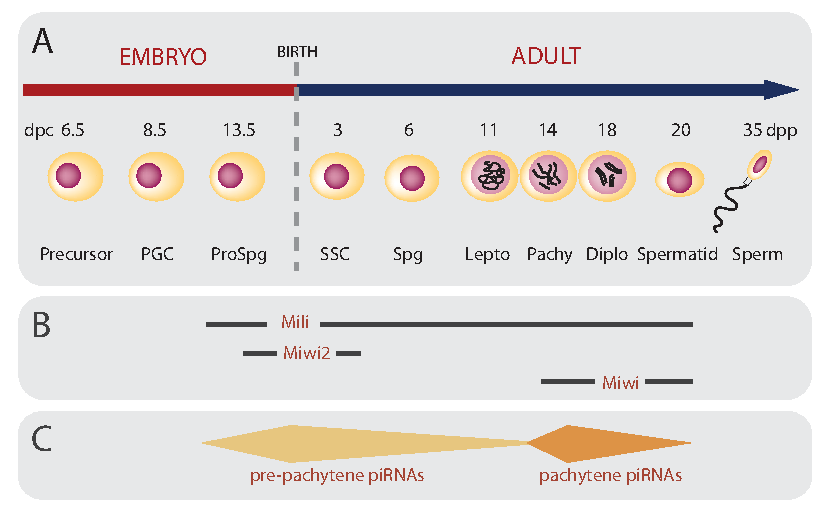
\includegraphics[width=14cm]{spermatogenesis}
\caption[Expression of piRNAs and PIWI proteins in spermatogenesis]{Expression of piRNAs and PIWI proteins in spermatogenesis. A) Formation of a mature sperm involves multiple differentiation steps in embryonic and adult development. Embryonic precursor cells of germ line develop 6.5 days \textit{post coitus} (dpc) and migrate to the gonads to form primordial germ cells (PGC). These then differentiate into male prospermatogonia (ProSpg) or gonadocytes before birth. Three days after birth (\textit{post par item} dpp), gonadocytes form spermatogonial stem cells (SSC), a testis specific pool of stem cells that differentiate into spermatogonia. Spermatogonia undergo mitosis to produce spermatocytes. These undergo meiosis, whereby chromosome condense in leptotene (Lept), recombine in pachytene (Pachy) and separate in diplotene (Diplo). After the second round of meiosis, round spermatids are formed which mature into sperm. B. Expression of Mili, Miwi and Miwi2 throughout the spermatogenesis. C. Production of pre-pachytene and pachytene piRNAs in relation to different stages of spermatogenesis and presence of PIWI proteins.}
 \label{fig:spermatogenesis}
\end{center}
\end{figure}


\subsection{piRNA biogenesis}
\label{sec:pingpong}
The biogenesis of piRNAs is related to its function in silencing of transposable elements (TEs) and occurs in three steps: transcription from mainly intergenic loci, export out of the nucleus and processing into oligonucleotides and amplification by the PIWI proteins \citep{Aravin:2006p384}. 

Initially, primary piRNAs transcripts are presumed to be transcribed from a set of genomic loci by an unknown RNA polymerase. Most piRNAs seem to map to the genome in clusters with a strand bias, pointing to biogenesis from long primary transcripts \citep{Aravin:2006p384}. These clusters are conserved in their chromosomal arrangement (synteny), but share no sequence similarity \citep{Girard:2006gu}. In mammals, there are several differences between the embryonic (pre-pachytene) and adult (pachytene) clusters. First, pre-pachytene and pachytene clusters show little overlap in their genomic loci. Second, the pachytene clusters contain a higher proportion of uniquely mapping piRNAs (80\% vs 60\%) and are depleted of transposable elements \citep{Betel:2007p580}. Finally, the majority of pachytene piRNAs are distributed over a smaller number of clustered regions, but with a greater concentration of piRNAs and a higher occurrence of sequence that are antisense to transposons \citep{Aravin:2006p384}. However, the current evidence for primary transcription is still only indirect and comes from mapping of piRNA sequences to their genomic locations.

The post-transcriptional steps of piRNA biogenesis are not well defined. It is presumed that single stranded primary transcripts are exported out of the nucleus and recognised by endo- and exonucleases such as Zucchini \citep{Nishimasu:2012cea, Ipsaro:2012ii}. Little is known about this step, except that processing probably occurs in perinuclear granules \citep{Siomi:2011gh}. Dicer has also been excluded from the process, since in \textit{D. rerio} it is not required for piRNA production and usually processes double stranded substrates \citep{Vagin:2006cs}.  After the processing by Zucchini that cuts specifically single-stranded piRNA precursors, the nascent fragments are taken by he PIWI proteins \citep{Siomi:2011gh}. Some PIWI proteins such as Ago2 in \textit{D. melanogaster} or Mili in mouse have a preference for the sequences with a first Uracil base  \citep{Brennecke:2007kf}. In the next step, the 3$\textprime$ end is trimmed by the exonucleases and methylated on the 2$\textprime$-O position to produce primary piRNAs. The current model does not account for the function of helicases (Armitage in \textit{D. melanogaster} and Mov10L1 in mouse) that are also required for piRNA biogenesis \citep{Saito:2010kq, Frost:2010jn, Zheng:2010ho}. 


\begin{figure}[hbtp!]
\begin{center}
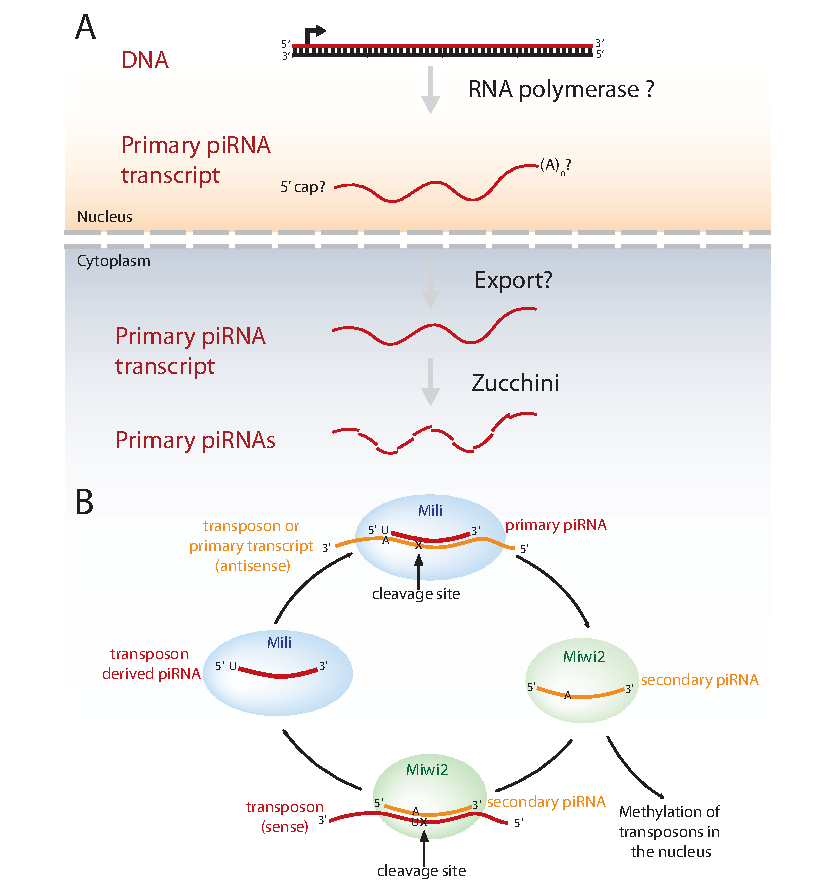
\includegraphics[width=14cm]{piRNAs}
\caption[Biogenesis of piRNAs]{The current model of mammalian piRNA biogenesis. Primary piRNAs prime Piwi proteins and guide them to transposon cleavage or methylation of transposon genomic loci. A. The primary precursors are transcribed by an unknown RNA polymerase and exported out of nucleus. The endonuclease Zucchini then cuts these single stranded piRNA precursors into oligonucleotides. B. The ``ping pong'' piRNA amplification cycle. The piRNAs with $5\textprime$ U are adopted by Mili that cleaves either the antisense transposon transcript or an antisense primary precursor. This cleavage event produces of a secondary piRNA with a tendency for 10' A. \citep{Brennecke:2008p641, Gunawardane:2007ka}. The secondary piRNAs target transposon RNAs that are generated from piRNA clusters. Cleavage of such transcripts reproduces original primary piRNAs that target antisense transposons or antisense primary transcripts. Miwi2 can also use the secondary piRNAs to target transposon loci in the nucleus.} 
 \label{fig:piRNAs}
\end{center}
\end{figure}

After the primary piRNAs have been formed, an amplification cycle termed ``ping-pong'' is supposed to create secondary piRNAs (Figure \ref{fig:piRNAs}). Sequencing of piRNAs revealed that the piRNAs on the opposite strands often overlap at their first 10 nucleotides, resulting in the propensity for U as the first nucleotide of a sense piRNA and A as the 10th nucleotide of a paired antisense piRNA. A mechanism was proposed by which Ago3 and Aub, two \textit{D. melanogaster} proteins in turn take piRNAs, cut transposon sequence, and use the nascent secondary piRNAs to cut more primary transcripts. The same mechanism was presumed in mice, with Mili and Miwi2 assuming the role of Ago2 and Aub \citep{Aravin:2007hw}.  By this model, Mili is primed by the piRNAs which are in the same sense as transposons. In combination with an unknown exonuclease to cut out the extra TE parts, this would create a secondary piRNA that commonly have Adenine at the 10th position. Since the sequences obtains from Miwi2 immunoprecipitations are enriched for these secondary piRNAs, it is presumed that it performs the second part of the cycle, by cutting the antisense transposon or primary piRNA transcript \citep{Aravin:2008kz}. This in turn would create more secondary piRNAs to cut transposons in an amplification loop. 
	The current ``ping pong'' model in mouse has several limitations. First of all, the �ping-pong� signature of 10 nt overlap between sense-antisense piRNA pairs is missing in adult testis \citep{Beyret:2012gc}. Second, Miwi2 is not present in the adult stages of spermatogenesis, when the pachytene piRNAs are being formed \citep{KuramochiMiyagawa:2008jn,Carmell:2007fi,Girard:2006gu}. Finally, Miwi2 is enriched in physically separate granules from Mili \citep{AlexeiAAravin:2009cu}.  


	\subsection{The function of piRNAs in mammals}
\label{piRNA_function}
The details of piRNA biogenesis have mostly been observed on embryonic piRNAs, while little is known on formation of the adult piRNAs. The same discrepancy applies to our knowledge of piRNA function during the course of spermatogenesis. 

The pre-pachytene piRNAs silence transposable elements (TEs)\nomenclature{TE}{transposable element}  in the embryonic stages of development. In animals  there are multiple types of TEs \citep{Jurka:1998vd}. The first ones are the Class I retrotransposons which contain an RNA during their cycle. Some of them form virus like particles in the cytoplasm and contain long terminal repeats (LTR)\nomenclature{LTR}{long terminal repeat}  that are used to insert their genetic sequences back into the host \citep{Shank:1978ub}. These LTRs, such as intracisternal A-particles (IAPs) \citep{Kuff:1983vj} contain a retrotransposase enzyme that allows for an increase in copy number by producing extra DNA copies from an RNA template \citep{Weiner:1986io}. Other Class I retrotransposons such as long and short interspersed nuclear elements (LINE and SINE)\nomenclature{LINE}{long interspersed nuclear element} \nomenclature{SINE}{short interspersed nuclear element} do not contain LTRs. LINE elements exit the cell and form ribonucleic particles, but SINEs do not code for proteins and use the machinery of LINE to increase the number of their copies. The class II or the DNA transposons \citep{Fraser:1983vn} code for a transposase \citep{Heffron:1979vza} that allows their movement around the genome, but they do not actively replicate. 

What all of the previously mentioned Class I transposons have in common is that they become active during the whole-genome demethylation that occurs during spermatogenesis \citep{Hajkova:2002ur, Walsh:1998cf}. The repression is mediated by piRNAs either by the endonucleolytic activity of PIWI proteins on transposon transcripts \citep{Aravin:2007hw} as described in Section \ref{sec:embryopingpong} or by silencing of their genomic regions through methylation of CpG islands \citep{KuramochiMiyagawa:2008jn}. Miwi2 performs methylation of TE genomic sites via a class of methylases called DNA methyltransferases (DNMT) \citep{Aravin:2008kz}. DNMT3L is a DNA methyltransferase that is germ line specific  and essential for methylation of transposons \citep{Bourchis:2004to}.

	Although the adult piRNAs were the first ones to be discovered, their biogenesis and function remain largely unknown. They are also formed from primary cluster loci, but their clusters are smaller, contain more piRNAs and are depleted of repeat regions \citep{Aravin:2007hw}. The details of their export and processing are also unknown and they seem seem to be amplified by the PIWI proteins \citep{Grivna:2006p577}. The non-repeat function of some piRNAs has been hypothesised to relate to chromatin, mainly through their involvement in the methylation process \citep{Olovnikov:2012ii}.  In \textit{D. melanogaster} clusters are often located in telomere and centromere regions, though their translocation to other regions did not have any effects on spermatogenesis \citep{Muerdter:2012jw}. A crucial step closer to identifying the function of pachytene piRNAs is to investigate the mechanism of their transcription and their evolution on a transcriptomic and epigenetic level (Chapter \ref{sec:chapter_piRNAs}). To that end, a set of sequence-based techniques has been employed, which will be discussed in the next section.


\section{Sequence-based technologies in genomics and transcriptomics}
\label{sequencing}
	Our current understanding of the biogenesis and function of non-coding RNA was largely possible due to the developments in the field of genomics. However, the path to the fully annotated genomes, such as the ENCODE\nomenclature{ENCODE}{encyclopaedia of human DNA elements} encyclopaedia of human DNA elements took several important steps. 
	
	The first genome sequenced was of $\Phi$X174 bacteriophage in 1977 \citep{Sanger:1977vp}. Genome size was a major technical limit and even small genomes such as  \textit{Escherichia coli} \citep{Blattner:1997ha} and \textit{Saccharomyces cerevisiae} \citep{Goffeau:1996eu} took a further 20 years to sequence. The first attempts to gain genome-wide information on  mammalian genomes was performed in 1990, with expressed sequence tags (EST) providing sequence information on 600 human protein-coding genes at once \citep{Adams:1991ua}. This information was used to build computational tools to annotate the next large sequencing endeavour, human chromosome 22 in 1997 \citep{Dunham:1999ib}, as a part of the Human Genome Project that started in the late 1980s \citep{Watson:1990ub}. The first draft of the human genome took more than 10 years before after the final version was publicly available and that required drastic changes in sequencing technology and gene prediction \citep{lander:2001hk}. 
	
	The focus then shifted to annotation of the genomic elements, which resulted in the ENCODE pilot project, annotating 1\% of the total human genome in 2007 \citep{Birney:2007fu}, and the full genome 5 years later \citep{Consortium:2012db}. The main techniques in analysis of sequence composition and gene expression that allowed for these scientific breakthroughs will be discussed in the next section.

	\subsection{Sequencing technologies}
	
	The principles of sequence-based technologies are grounded in the properties of nucleic acids that make them efficient information carriers \citep{Church:2012fd}. The first one is the accurate information transfer from one strand of DNA or RNA to the complementary one, due to the rules of base pairing. The second is the easy information amplification for increased signal-to-noise ratio, due to the ability of double strands of DNA to separate and re-hybridise under high-low temperature cycles or enzymatic treatment. These two properties in combination with various protein catalysts and chemically modified nucleotides are still the basis for the majority of methods for sequence identification and quantification \citep{Morozova:2008cn}.

	\subsubsection{The early days}
	\label{PCR}
	
	Maxam and Gilbert were the first to develop a method for DNA sequencing in 1977 \citep{Maxam:1977vy}. Their method involved separation of a sample into four parts and incomplete chemical degradation of one out of four nucleotides in each of the subsamples. This was followed by the separation of resulting $5\textprime$ radioactively labeled DNA fragments on a polyacrylamide gel, whereby fragment length pointed to the position of individual nucleotides in the sequence. Similarly, the Sanger method used the length of fragments created by DNA polymerase, with four different dideoxy nucleotide homologues stopping the polymerisation at their inclusion sites \citep{Sanger:1977vp}. Furthermore, modifications of the Sanger method were later developed, whereby different fluorescent dyes were tagged to the dideoxy nucleotides themselves \citep{Smith:1986ie}. This approach allowed for automation of the process by combining the four subsamples for each nucleotide, and detecting the fluorescent colour of each of the fragment band as it passed through a high sensitivity fluorescence detector. The sequence was determined from the temporal order of peaks corresponding to each of four different fluorescent dyes, and the computers were used to deconvolute the signal. Finally, the sequencing was further speeded up and automated by use of capillary electrophoresis instead of gels, which allowed for parallel analysis of up to 96 samples \citep{Blattner:1997ha}.  
	
	\subsubsection{Second generation sequencing}
	\label{sgs}
	The previous approaches were used to sequence genomes of major model organisms, from Bacteria \citep{Blattner:1997ha} to human \citep{lander:2004bm}, but it was the development of modern techniques of �second� or �next� generation sequencing that allowed for a drastic increase in sequencing speed and reduction in cost \citep{Metzker:2009ew}. These methods do not evaluate sequence composition by fragment sizes, but by the individual polymerisation additions for each of the nucleotides to the complementary strand of sequenced DNA. 
	
	The first method was pyrosequencing, developed in 1996 \citep{Ronaghi:1996jt}. Sample DNA with adapter sequences were added to streptavidin-coated magnetic beads in quantities that promoted ligation of only one sequence to a bead. The template on each bead was then amplified through a polymerase chain reaction (PCR)\nomenclature{PCR}{polymerase chain reaction}  (see Chapter \ref{PCR}). In the next step, each of the four nucleotides were added and removed in turn, in the presence of a mixture of enzymes required for the DNA polymerase reaction and photo-detection. Successful incorporation of a nucleotide releases a pyrophosphate which activates a photo-reactive moiety in a quantitative manner \citep{FakhraiRad:2002ke}. This methodology is the basis for the commonly used 454 sequencing system, whereby the individual beads with a sample are spread over small wells and individually pyrosequenced, allowing for genome-scale analyses \citep{Margulies:2005gw}. 
	
	The Illumina method shares this ``sequencing by synthesis'' approach with 454 technology, but several differences have made it more popular. The sequencing is performed on solid surfaces, not  beads, and this allows for a much larger number of sequences to be evaluated in parallel \citep{Bentley:2008eo}. This is achieved by initial attachment of DNA randomly to a flow cell, followed by amplification that creates clusters of up to 1000 identical DNA sequences. Next, the nucleotides are added in turn, but unlike 454 where incorporation of copies of a nucleotide in the same cycle are a possible source of error, the Illumina system uses nucleotides as polymerisation terminators. This ensures that only a single nucleotide can be incorporated in time. The attached fluorescent dyes are then detected by the instrument for each cycle of synthesis. Furthermore, the initial limit of 18 gigabases (Gb) per Illumina Genome Analyzer run \citep{Metzker:2009ew} was increased to 600 Gb for the HiSeq method, with the maximum length of reads now at 100 bp \citep{Liu:2012hw}. This is several orders more processive than 454 (0.45 Gb per run), but the length of 454 reads (330 nt) allows for better assessment of sequenced regions with gaps and repeats \citep{Metzker:2009ew}. 
	
	Finally, SOLiD sequencing is the third largest sequencing platform. Instead of using sequencing by synthesis, it performs DNA sequencing based on ligation of fluorescently labeled probes to the DNA sequence \citep{McKernan:2009cl}. After amplification of sequences on beads similar to 454, the beads are deployed on flow cells. A complex set of overlapping primers is then added to guide the binding of probes, labeled based on the nucleotide content of their first two bases. Ultimately, for each nucleotide of the sequence two nucleotides are assessed at the time, whereby each nucleotide is effectively sequenced twice. This allows for higher accuracy of detected sequences, which makes this technology more suited for variation studies. However, the time required for sequencing is on the order of weeks and the reads are shorter than in the other methods (50 bp) \citep{Liu:2012hw}. 
	
	\subsubsection{Applications of the second generation sequencing methods}
	\label{SGS_applications}
	
	The decreasing cost of the sequencing methods allowed for their wide usage beyond pure sequence determination and a selected few will be discussed in more detail.
	
	RNA-seq experiments allow for a quantitative assessment of the amount of gene expression as well as the detection of novel transcripts. The technology is based on extraction of RNAs either by poly(A)-enrichment or rRNA depletion of total cellular RNA content, followed by cDNA synthesis and second generation sequencing \citep{Morin:2008gf}. The number of sequences detected can be used to estimate a broad range of transcript expression, while in the same time detecting both coding and non-coding transcripts. 
	
	ChIP-seq (CHromatin ImmunoPrecipitation followed by sequencing)\nomenclature{ChIP-seq}{chromatin immunoprecipitation followed by sequencing}  technology has been widely used in the fields of expression regulation and epigenetics, since it detects the DNA-protein interaction sites of DNA-binding proteins \citep{Barski:2007gh}. In the first step of this methodology proteins are crosslinked with bound DNA, typically with formaldehyde. This is followed by immunoprecipitation of the target protein, and sequencing of the unlinked DNA with second generation sequencing. 
	
	Furthermore, these methods can also be used to detect interactions of close fragments of DNA, with a range of techniques jointly known as ``chromosome conformation capture'' \citep{Dekker:2002ub}. These techniques are also based on crosslinking of DNA strands with proteins, although this time a protein is involved in interaction with two DNA sequences. The treatment of such DNA-proteins complexes with a restriction enzyme digestion leaves short sequences attached to a protein.  In the next step, these short sequences are ligated and detached from the protein. The initial methods such as  3C \citep{Dekker:2002ub}, 4C \citep{Zhao:2006jn} and 5C \citep{Dostie:2006kx} amplified the ligated DNA with specific primers, allowing for identification of DNA interactions of only specific loci. However, the recently developed HiC \citep{LiebermanAiden:2009jz} protocol captures DNA-DNA interactions on a genome-scale level. The specificity of capturing only crosslinked DNA is achieved by using biotin in the ligation step, and is followed by a capture with spretavidin, second generation sequencing and a complex computational analysis. 
	
	Finally, the bisulfite sequencing method captures the methylation state of a genome \citep{Ball:2009kh}.  Addition of a methyl group to cytosine residues of the CpG dinucleotides has been implicated in transcriptional repression. Treatment of DNA with bisulfite introduces specific changes by converting non-methylated Cytosine residues to Uracil. After sequencing, these changes that point to methylation sites can be observed by a comparison with the original genomic sequence. 
			
	\subsubsection{Third generation sequencing}
	
Despite their broad usage, current sequencing methods have several inherent problems. They depend on PCR amplification of sequences to clusters, either on beads or flow cells, which introduces further biases and reduces complexity of the sample  \citep{Schadt:2010cp}. Furthermore, they produce large quantities of redundant, overlapping data with sequences of short length. In the last few years there has been a decrease in the time and cost of sequencing \citep{Metzker:2009ew, Liu:2012hw}, but single molecule sequencing (SMS) techniques are expected to bring it down even more \citep{Pushkarev:2009cw}. SMS intends to acquire sequence information from a single molecule of DNA or RNA as it passes through a detector in multiple ways. The Helicos system images polymerisation of the second strand in real time with a defined primer, a modified polymerase and fluorescently labeled nucleotide analogues, producing short reads of 25 nt \citep{Harris:2008gf}. Single molecule real time sequencing (SMRT) by Pacific Biosciences directly observes polymerisation of a single molecule of DNA by observing the release of a fluorescent dye as it leaves the tiny polymerisation chamber \citep{Eid:2009kv}. Finally, the Oxford nanopore system detects individual nucleotides once they are cleaved from the individual DNA molecules and pass through small pores. All of these technologies are still in development, but once technical issues are solved the low cost that they promise and the amount of the sample needed will likely allow them to dominate the field of nucleic acid sequencing

	\subsection{Gene expression profiling}

The previously mentioned sequencing approaches provide mostly just the bare sequence of the DNA or RNA in question. The second generation sequencing crossed this line from the qualitative to quantitative analysis of sequences, since the number of times a sequence appears in the output can be used as a measure of the abundance of the template sequence. However, the majority of gene expression quantification is still performed with non-sequencing technologies due to their low cost and the well established analysis protocols.

	\subsubsection{The early days}

	The first technique to evaluate gene expression levels was the Northern blot, developed in late 1970s \citep{Alwine:1977uz}. The procedure involved separation of mRNAs based on their size with gel electrophoresis, followed by hybridisation of radioactively fluorescently tagged oligonucleotide probes for the sequence of interest. The technique allows for both qualitative and quantitative evaluation of expression, and is still in use today for its simplicity. In 1983 the polymerase chain reaction (PCR) method was developed that revolutionised molecular biology by allowing for amplification of minute amounts of genetic material \citep{Saiki:1985to, Mullis:1990wx}. The PCR reaction amplifies DNA or RNA by using thermostable polymerases that remain active despite multiple cycles at room temperature ssDNA-primer annealing and dsDNA polymerisation and high temperature and dsDNA separation (``melting''). PCR can be used to detect expression through the use of quantitative real-time PCR (qRT-PCR) technique \citep{Holland:1991tc}. In these methods, a dye is added that fluoresces upon binding to dsDNA, or the degradation of a part of probe releases an otherwise quenched fluorophore. The amount of fluorescence is then compared to a control for each cycle, or a relative amount to an internal reference gene can be measured. Despite being the gold standard to measure RNA expression even today, the major drawback is its inability to measure expression of all cellular transcripts at once.

	\subsubsection{High throughput methodologies}
	\label{microarrays}
	The first step in evaluation of gene expression on a genome scale level was the introduction of expressed sequence tags (EST) in the 1990s \citep{Adams:1991ua}. ESTs are small DNA sequences (300-500 nucleotides long) generated by sequencing total mRNA of all expressed genes in cells of interest. Messenger RNAs were first converted to complementary DNA (cDNA)\nomenclature{cDNA}{complementary DNA}  with an enzyme reverse transcriptase and then sequenced from both the $5\textprime$ and $3\textprime$ end. This technique allowed, for the first time, cataloguing of species and tissue specific transcriptomes. Furthermore, the unique ESTs were the basis of the Unigene database, that contains unique identifiers for all the known genes \citep{Boguski:1995kg}. Finally, besides being an early gene finding tool, the EST libraries were also used for the first two whole genome expression platforms; serial analysis of gene expression (SAGE) and DNA microarrays.
	
 	SAGE is a genome wide expression assessment platform that can provide information on all expressed mRNA in a sample at once \citep{Velculescu:1995ik}. In the first step, small sequence tags (\textless30 bp) are obtained from $5\textprime$ or $3\textprime$ part of the expressed transcript. Next, the tags are concatenated together and sequenced. In the final step the expression level of each transcript is quantified based on the frequency of each of the observed tags. With the help of EST libraries, expression of individual genes was assessed, but this technique was soon replaced by cheaper and less labour intensive DNA microarrays.
	
	Despite the rise of second generation sequencing methods, DNA microarrays (or DNA chips) still provide a robust approach in evaluation of mRNA expression \citep{Malone:2011ib}. The method is based on binding of a sample of mRNAs to complementary cDNA or ssDNA  oligomers (probes) that were previously attached to a solid glass or plastic surface \citep{Schena:1995tu}. There are several modifications to the basic idea. In the two-sample protocol, short complementary cDNA of interest is spotted on arrays and bound by two samples that are tagged with either green or red fluorescent marks. The ratio of green to red fluorescence evaluates relative amounts of expressed mRNA for each of the samples \citep{Shalon:1996uf}. In the second type, the oligonucleotide microarrays, the probes are synthesised on a silicon or glass surface (array or chip) and are 60 (Agilent) \citep{Blanchard:1996go} or 25 (Affymetrix) \citep{Lipshutz:1999ez} nucleotides long.  In this approach, the mRNA sequences are added to the oligonucleotide samples without a second color, and their expression is compared across conditions. The accuracy of binding is measured against binding to oligonucleotides with a mismatch in the middle of the sequence. The third approach is used is the BeadArray technology \citep{Oliphant:2002vf}. In this approach the probes are attached to beads, and deployed randomly on arrays to be bound by labeled complementary RNA (cRNA). The detection of the probe location is performed through a specific 29 nt ``address'' at the $5\textprime$ end of the probe.  
	
	In summary, microarrays are still the method of choice for the evaluation of the coding transcripts, since they are the statistically well defined system and inexpensive compared to the sequencing technologies \citep{Malone:2011ib}. However, the problem is that they can only detect previously described sequences (usually protein-coding ones) and are not capable to detect novel transcripts. Furthermore, they cannot be used to quantify absolute gene expression, but can only provide an expression value relative to a reference sample.  A modification of the DNA microarrays called tiling arrays circumvents this problem by placing on multiple chips oligomeric sequences that cover an entire genome \citep{Bertone:2004gj}. Tiling arrays have been used in multiple other methods: to detect regions bound by immunoprecipitated DNA-binding proteins (chip-ChIP) \citep{Horak:2002uj}, chromatin methylation (MEDip-ChIP) \citep{Palmke:2011hz} or chromosomal duplications in cancer (CGH)\citep{Pinkel:1998da}. However, despite the statistical power and multiple applications, the cost of tiling arrays for mammalian genomes is prohibitive, where they are already replaced by the second generation sequencing methods.

\nomenclature{ssDNA}{single stranded DNA} 
\nomenclature{dsDNA}{double stranded DNA} 
\nomenclature{ssRNA}{single strandedRNA} 
\nomenclature{dsRNA}{double stranded RNA} 

\newpage
\section{Aims of the analyses}

During the course of my studies, my aim was to investigate properties of non-coding RNAs from a perspective of computational biology. Three types of RNAs were the focus of method development and data analysis: pachytene piRNAs, pre-pachytene piRNAs and microRNAs. 

Unlike pre-pachytene piRNAs, which are largely involved in the regulation of mobile genetic elements, the function of the pachytene piRNAs remains elusive \citep{Siomi:2011gh}. These piRNAs are associated with Mili and Miwi only, and are expressed later in spermatogenesis in exceptionally large amounts \citep{Aravin:2006p384}. They seem to contribute greatly to the germinal granules or nuage where they are stored together with other haploid mRNA transcripts \citep{Meikar:2010jm}. Most pachytene piRNAs seem to be produced from long primary transcripts \citep{Aravin:2006p384}, but little is know about their transcription properties as well as their mechanism of formation.
The aim of this aspect of my studies was to define genomic features and evolutionary mechanisms underlying mammalian germ-line-specific noncoding RNAs. To that end, I have analysed datasets of multiple experiments on RNA polymerases and major histone marks in the testes and livers of mouse, dog and opossum. 

Biogenesis of embryonic piRNAs in mouse is better defined than the pachytene ones. The production of these pre-pachytene piRNAs is considered dependent on PIWI proteins Mili and Miwi2 \citep{Aravin:2008kz}. These two proteins direct silencing of LINE1 and IAP transposons on both expression and epigenetic level. The mouse model of biogenesis presumes a circular amplification between Mili and Miwi2 for two major transposable elements similar to \textit{D. melanogaster}. In order to investigate the role of endonucleolytic activity of Piwi proteins in this process,  engineered point mutations were introduced in mice that substitute the second D to an A in the catalytic triad (DDH) of Mili and Miwi2, generating the Mili\textsuperscript{DAH} and Miwi2\textsuperscript{DAH} alleles, respectively. The aim of the second project was to design a pipeline for pre-pachytene piRNA analysis and to assess the contributions of Mili and Miwi2 endonucleolytic activities to the production of pre-pachytene piRNAs.

While the previous project focused on piRNAs, the final project addressed the issue of detection of miRNA targeting in experimental datasets. The current computational target prediction tools use several features of miRNAs that range from sequence properties and conservation to thermodynamic energy. Instead of using the feature approach to target prediction, one can attempt to detect targets by observing the influence of miRNAs on global expression profiles \citep{Lim:2005cd}. Using that approach, the Sylamer algorithm has been developed in the group of Anton Enright \citep{vanDongen:2008cb}. Sylamer finds significantly over- or underrepresented words of specific length in the $3\textprime$ UTRs of ranked gene lists. It calculates the significance of each word being more abundant than expected at one end of the list compared to the rest, using the hypergeometric distribution. The final aim of my PhD was to build a system for an automated, fast and reliable assessment of miRNA influence on expression datasets based on the Sylamer algorithm. 
%%% ----------------------------------------------------------------------


%%% Local Variables: 
%%% mode: latex
%%% TeX-master: "../thesis"
%%% End: 
